\subsection{Inference: Efficient Sampling with EDM--Heun}
\label{sec:recipe-inference}

\textbf{Explored designs.}
We compare flow ODE with Euler integration, flow SDE with Euler--Maruyama, and
EDM--Heun~\citep{karras2022elucidating} at matched numbers of function
evaluations (NFE), and sweep the EDM discretization exponent $\rho$. For
template conditioning, we compare random rotation and translation, rotation
only, and no augmentation at inference to test whether reducing template
randomness improves performance. Finally, we evaluate
autoguidance~\citep{karras2024guiding}, using earlier training checkpoints as
degraded models following \citet{geffner2025proteina}.

\textbf{Results and selection.}
At 400 NFE, EDM--Heun achieves $\mathrm{Sol}_C=0.482$, compared with $0.430$
for flow SDE and $0.408$ for flow ODE. Increasing EDM--Heun from 400 to 1000
NFE improves $\mathrm{Sol}_C$ by only $0.005$, so we retain 400 NFE.
Performance is similar for $\rho\in[5,10]$; following
\citet{karras2022elucidating}, we select $\rho=7$. Reducing template
augmentation does not improve performance, with all three variants reaching
$0.485$--$0.487$, so we retain the training-matched rotation and translation.
Autoguidance also provides no benefit: the best guided setting reaches $0.470$,
compared with $0.487$ without guidance. We therefore select EDM--Heun at 400 NFE with
$\rho=7$, template rotation and translation, and no autoguidance.

\begin{figure}[!t]
  \centering
  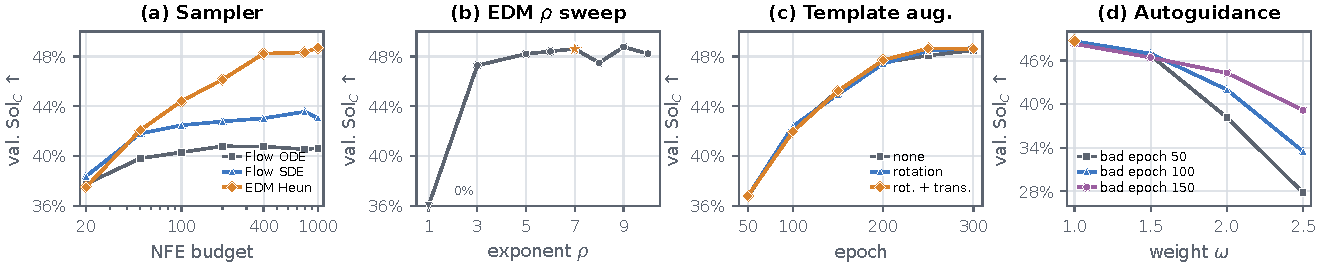
\includegraphics[width=\textwidth]{figures/generated/fig_inference_sweeps.pdf}
  \caption{\textbf{Inference ablations.}
    \textbf{(a)} Validation $\mathrm{Sol}_C$ versus NFE budget for flow ODE,
    flow SDE, and EDM--Heun. \textbf{(b)} EDM--Heun with 400 NFEs across
    discretization exponents $\rho$; the failed $\rho=1$ result is shown at the
    lower boundary, and the star marks the selected $\rho=7$.
    \textbf{(c)} Validation trajectories with no template augmentation,
    rotation only, and rotation plus translation at inference.
    \textbf{(d)} Autoguidance using degraded checkpoints from epochs 50, 100,
    and 150 across guidance weights $\omega$.}
  \label{fig:inference-sweeps}
\end{figure}
